\paragraph{arithmetic\_base}

ArithmeticGate is a gate which can perform a weighted multiply-add, i.e.
\[ \text{res} = \text{cons\_0} \times \text{mul\_0} \times \text{mul\_1} + \text{cons\_1} \times \text{add}. \]

The structure of gate is shown in \figref{fig:arithmetic-gate}.

\begin{figure}[!ht]
    \centering
    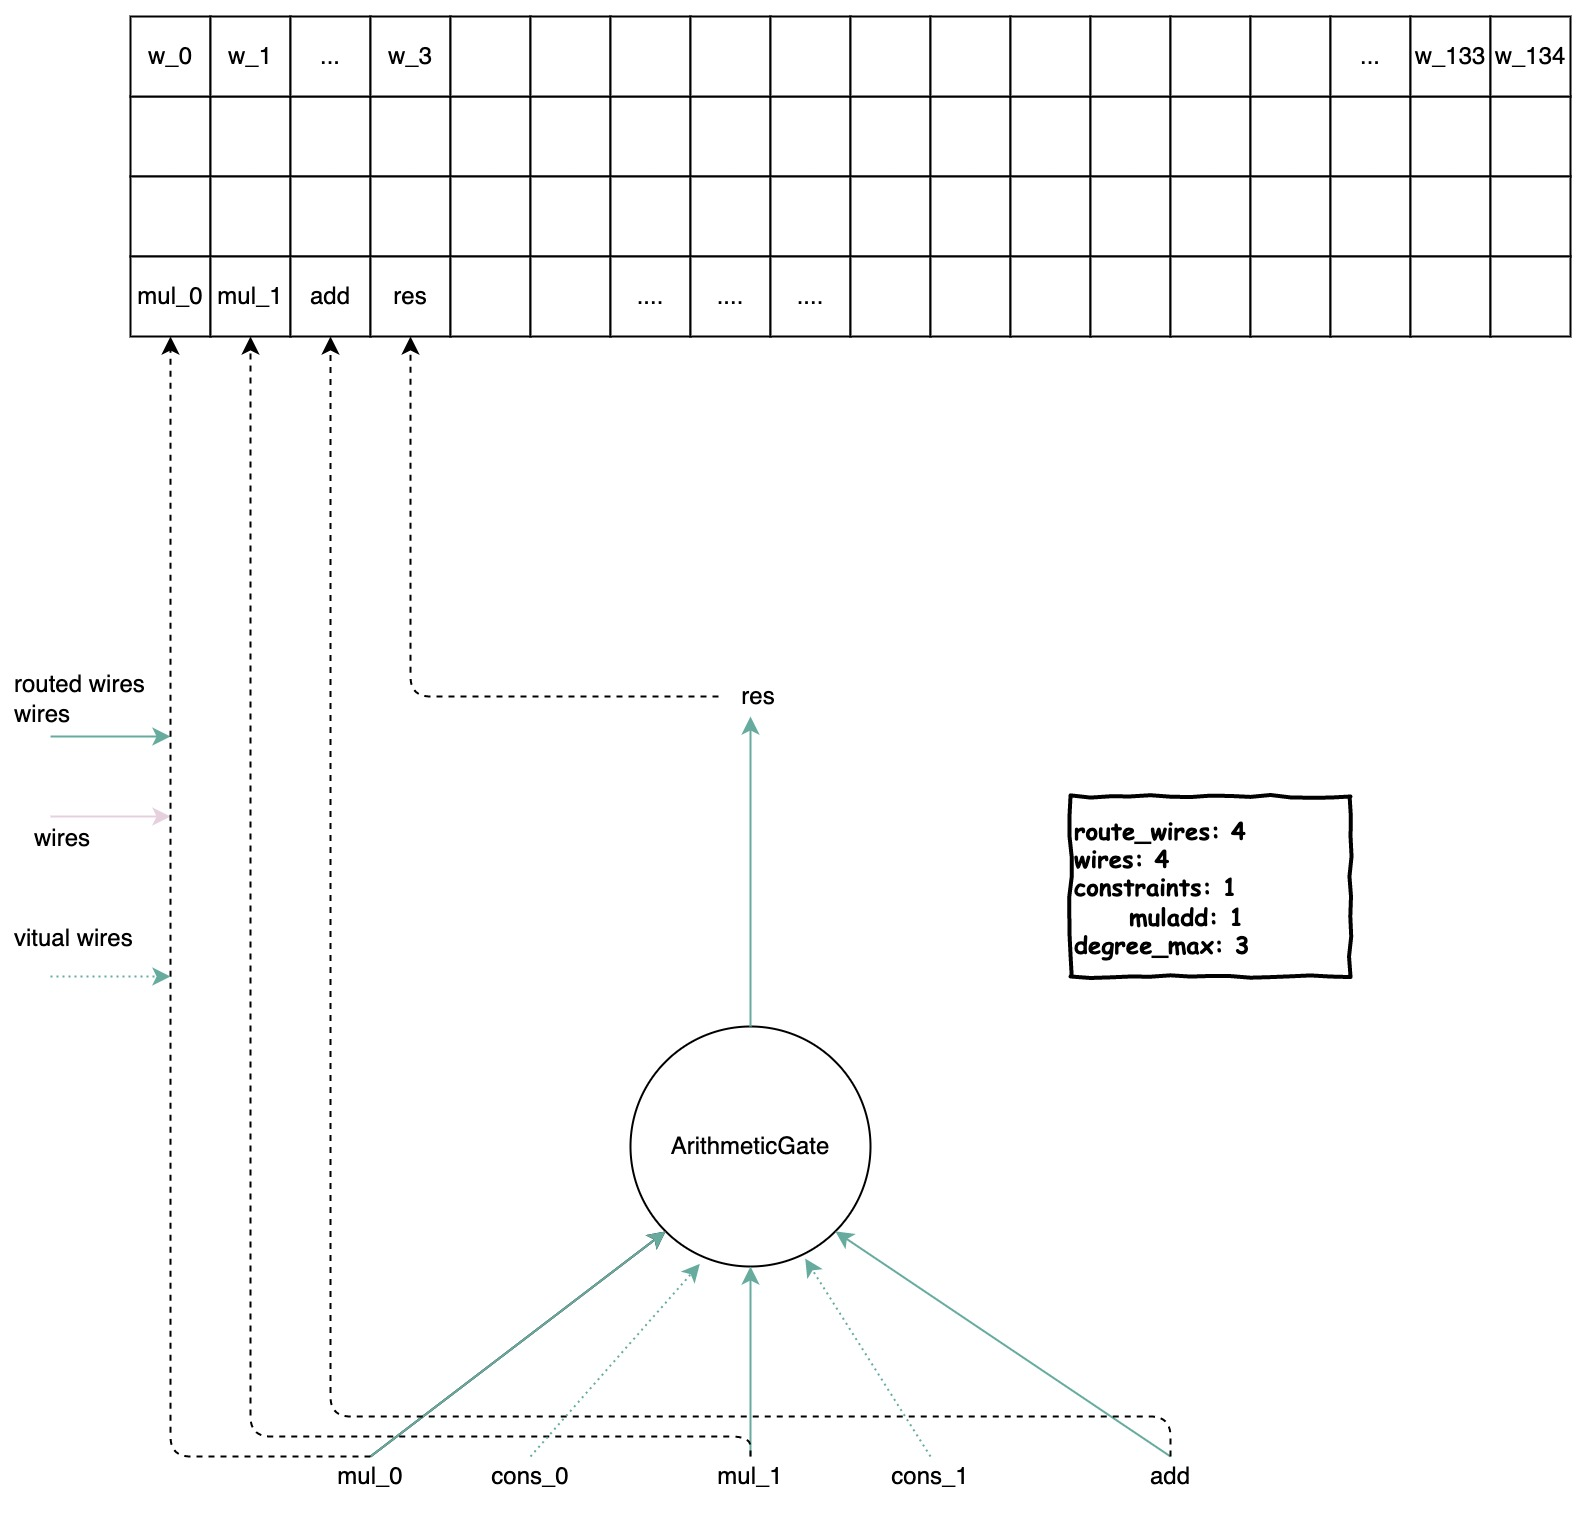
\includegraphics[width=0.5\textwidth]{gates/arithmetic_base.jpeg}
    \caption{ArithmeticGate}
    \label{fig:arithmetic-gate}
\end{figure}

There's only one constraint per operation, and degree is 3.
